\documentclass[../DoAn.tex]{subfiles}
\begin{document}
Trong chương này, tôi sẽ tập trung vào việc khảo sát và phân tích yêu cầu của đề tài. Đầu tiên, tôi tiến hành khảo sát các công nghệ, thiết bị và giải pháp liên quan, nhằm thu thập các thông tin cần thiết phục vụ cho việc phát triển hệ thống. Tiếp theo, dựa trên kết quả khảo sát, tôi sẽ phân tích các hướng giải quyết khả thi, từ đó đề xuất phương án thực hiện phù hợp nhất cho đề tài.

\section{Khảo sát hiện trạng}
\label{section:2.1}
Phần này sẽ trình bày tổng quan khảo sát về một số hạn chế của các hệ thống theo dõi hiện nay.
\subsection{Hạn chế của các hệ thống hiện tại}
\label{subsection:2.1.1}
Hiện nay, các hệ thống giám sát GNSS (Global Navigation Satellite System) được ứng dụng rộng rãi trong nhiều lĩnh vực như giám sát phương tiện, quản lý đội xe, và định vị cá nhân. Tuy nhiên, các hệ thống này vẫn còn tồn tại nhiều hạn chế, ảnh hưởng đến độ chính xác và tính ổn định trong quá trình vận hành.

Một trong những hạn chế lớn nhất của các hệ thống GNSS hiện tại là độ chính xác bị ảnh hưởng bởi nhiều yếu tố ngoại cảnh. Tín hiệu vệ tinh có thể bị nhiễu do các tác động môi trường như thời tiết xấu, địa hình phức tạp (đồi núi, hẻm sâu), hoặc các vùng đô thị với mật độ cao. Điều này dẫn đến sai số định vị, ảnh hưởng trực tiếp đến khả năng giám sát liên tục và đáng tin cậy của hệ thống.

Một vấn đề đáng lo ngại khác là khả năng bị tấn công giả mạo tín hiệu GNSS. Các tín hiệu giả mạo có thể được tạo ra từ các thiết bị phát sóng trái phép (spoofing), làm cho hệ thống giám sát nhận diện sai vị trí thực tế. Điều này gây ra những hậu quả nghiêm trọng trong các ứng dụng yêu cầu độ chính xác cao như giám sát an ninh, quản lý giao thông, hoặc theo dõi phương tiện công cộng.

Các hệ thống GNSS hiện tại thường khó tích hợp với các nền tảng IoT hiện đại do khác biệt về giao thức truyền thông và cách thức xử lý dữ liệu. Việc truyền dữ liệu GNSS lên các nền tảng IoT để giám sát và phân tích thời gian thực thường yêu cầu xử lý trung gian phức tạp, dẫn đến độ trễ trong việc hiển thị vị trí và trạng thái di chuyển.

Trong các hệ thống giám sát di động, việc duy trì giám sát GNSS liên tục tiêu thụ một lượng năng lượng đáng kể. Điều này làm giảm thời gian hoạt động của thiết bị, đặc biệt trong các ứng dụng di động hoặc khi sử dụng các thiết bị IoT với nguồn pin hạn chế.

Nhìn chung, các hệ thống giám sát GNSS hiện tại còn nhiều hạn chế về độ chính xác, khả năng chống giả mạo, tích hợp với hệ thống IoT, và hiệu năng năng lượng. Để khắc phục các vấn đề này, cần có những giải pháp cải tiến cả về mặt công nghệ định vị lẫn tích hợp hệ thống, từ đó đảm bảo hệ thống giám sát GNSS đạt hiệu quả cao và đáp ứng được các yêu cầu thực tiễn.
\subsection{Các yêu cầu chức năng của hệ thống}
\label{subsection:2.1.2}
Hệ thống giám sát GNSS và geofence cần đảm bảo khả năng giám sát liên tục để đáp ứng các yêu cầu theo dõi vị trí theo thời gian thực. Điều này đòi hỏi hệ thống phải liên tục thu thập và xử lý dữ liệu định vị từ thiết bị, đồng thời truyền tải lên nền tảng ThingsBoard một cách ổn định. Các thông tin như tọa độ, tốc độ di chuyển và trạng thái kết nối phải được cập nhật tức thời, tránh tình trạng mất tín hiệu hoặc gián đoạn, đảm bảo hệ thống có thể theo dõi và giám sát liên tục các đối tượng được quản lý.

Bên cạnh đó, tính năng geofence là một trong những yêu cầu quan trọng của hệ thống. Hệ thống cần cung cấp khả năng thiết lập các vùng giám sát địa lý trên bản đồ, xác định ranh giới khu vực mà đối tượng được phép di chuyển. Khi đối tượng ra khỏi vùng geofence hoặc di chuyển vào khu vực không được phép, hệ thống cần ngay lập tức phát hiện và gửi cảnh báo tới người quản lý. Việc thiết lập, thay đổi hoặc xóa vùng giám sát phải được thực hiện một cách linh hoạt, dễ dàng từ giao diện quản lý.

Ngoài ra, hệ thống cần tích hợp tính năng cảnh báo tự động khi đối tượng di chuyển vượt quá ranh giới geofence. Điều này giúp người dùng kịp thời phát hiện các tình huống bất thường hoặc vi phạm khu vực giám sát. Các cảnh báo cần được gửi dưới dạng thông báo tức thời qua các kênh như tin nhắn, email hoặc qua nền tảng ThingsBoard, giúp người quản lý nhanh chóng đưa ra các biện pháp xử lý.

Hệ thống cũng cần đảm bảo khả năng lưu trữ và quản lý lịch sử di chuyển của đối tượng trong một khoảng thời gian nhất định. Dữ liệu lịch sử cần được tổ chức và truy xuất dễ dàng, hỗ trợ việc phân tích hành trình, đánh giá hiệu quả giám sát, cũng như phục vụ công tác quản lý và báo cáo. Điều này đòi hỏi hệ thống phải có cơ chế lưu trữ dữ liệu an toàn, với dung lượng đủ lớn để đáp ứng nhu cầu sử dụng lâu dài.
\subsection{Các yêu cầu phi chức năng của hệ thống}
\label{subsection:2.1.3}
Để đảm bảo hiệu quả trong quá trình vận hành, hệ thống giám sát GNSS và geofence cần đáp ứng các yêu cầu phi chức năng về hiệu năng xử lý và tiêu thụ năng lượng. Hiệu năng của hệ thống phải đảm bảo khả năng thu thập và xử lý dữ liệu định vị theo thời gian thực mà không gây ra độ trễ lớn. Điều này đặc biệt quan trọng trong các ứng dụng giám sát liên tục như theo dõi phương tiện hoặc giám sát an ninh. Đồng thời, hệ thống cần tối ưu hóa tiêu thụ năng lượng, nhất là đối với các thiết bị di động hoặc IoT sử dụng nguồn pin. Việc giảm thiểu tiêu thụ năng lượng giúp kéo dài thời gian hoạt động của thiết bị, hạn chế việc gián đoạn do hết pin.

Một trong những yêu cầu phi chức năng quan trọng khác là bảo mật dữ liệu và chống giả mạo tín hiệu GNSS. Hệ thống cần đảm bảo rằng các dữ liệu định vị được thu thập và truyền tải đều được mã hóa, bảo vệ trước các tấn công mạng như giả mạo vị trí (spoofing) hoặc can thiệp tín hiệu (jamming). Các cơ chế phát hiện tín hiệu bất thường cần được tích hợp, đảm bảo việc giám sát không bị sai lệch do các cuộc tấn công có chủ đích. Việc bảo mật này giúp đảm bảo tính toàn vẹn và độ tin cậy của dữ liệu thu thập được.

Hệ thống cũng cần có tính tương thích cao với các nền tảng IoT hiện đại, đặc biệt là trong việc tích hợp với ThingsBoard để quản lý thiết bị và giám sát từ xa. Việc sử dụng các giao thức truyền thông phổ biến như MQTT giúp tăng cường khả năng tương tác giữa các thiết bị và nền tảng. Điều này tạo điều kiện thuận lợi cho việc triển khai trên nhiều môi trường khác nhau mà không gặp phải các vấn đề tương thích.

Cuối cùng, tính ổn định và độ tin cậy là yếu tố quan trọng trong mọi hệ thống giám sát. Hệ thống cần hoạt động liên tục, ổn định trong thời gian dài mà không gặp phải sự cố hoặc mất tín hiệu. Việc giám sát và tự động khôi phục trong trường hợp lỗi giúp giảm thiểu tác động tiêu cực khi hệ thống bị gián đoạn. Các phương thức kiểm tra, bảo trì và nâng cấp định kỳ cũng cần được thiết lập rõ ràng, giúp duy trì hiệu năng ổn định trong suốt vòng đời của hệ thống.
\section{Phân tích hướng giải quyết}
\label{section:2.2}
Sau khi đã khảo sát và tìm hiểu các hệ thống giám sát GNSS hiện tại cũng như các yêu cầu cần thiết, chương này sẽ tập trung vào việc phân tích các hướng giải quyết nhằm xây dựng một hệ thống giám sát GNSS và geofence hiệu quả, đáp ứng các yêu cầu kỹ thuật đã đề ra.

Phần này sẽ trình bày mô hình hệ thống với các thành phần chính, từ đó xác định vai trò và chức năng của từng thành phần trong quá trình giám sát. Tiếp theo, việc lựa chọn công nghệ và nền tảng sẽ được phân tích kỹ lưỡng để đảm bảo hệ thống đạt được hiệu năng cao, tối ưu hóa năng lượng, và có khả năng chống giả mạo tín hiệu GNSS.

Bên cạnh đó, chương cũng sẽ đánh giá tính khả thi của các giải pháp đề xuất, dựa trên các tiêu chí như độ chính xác, độ tin cậy, khả năng mở rộng và tích hợp với các nền tảng IoT. Kết quả của quá trình phân tích này sẽ làm cơ sở để tiến hành thiết kế và triển khai hệ thống trong các bước tiếp theo.
\subsection{Mô hình hệ thống}
\label{subsection:2.2.1}
Để xây dựng một hệ thống giám sát hiệu quả, đáp ứng các yêu cầu về giám sát liên tục, và quản lý vị trí theo thời gian thực, mô hình hệ thống cần được thiết kế với cấu trúc rõ ràng, tích hợp các thành phần chính một cách hợp lý để đảm bảo khả năng thu thập, xử lý và truyền tải dữ liệu định vị.

Hệ thống giám sát GNSS và geofence bao gồm ba thành phần chính: thiết bị giám sát, hệ thống trung tâm xử lý dữ liệu và nền tảng hiển thị thông tin. Thiết bị giám sát được lắp đặt trên đối tượng cần theo dõi, có chức năng thu thập tín hiệu vệ tinh để xác định vị trí hiện tại. Thiết bị này cần tích hợp các module GNSS hiện đại, đồng thời có kết nối mạng để truyền dữ liệu về trung tâm.

Hệ thống trung tâm xử lý dữ liệu đóng vai trò quan trọng trong việc thu thập, phân tích và lưu trữ dữ liệu định vị. Dữ liệu từ thiết bị GNSS được truyền về trung tâm thông qua các giao thức truyền thông như MQTT hoặc HTTP. Tại đây, dữ liệu được xử lý để phát hiện các sự kiện bất thường như mất tín hiệu hoặc di chuyển ra ngoài vùng geofence. Hệ thống xử lý cần có khả năng phân tích dữ liệu nhanh chóng, đảm bảo độ trễ tối thiểu khi xử lý tín hiệu định vị.

Nền tảng hiển thị thông tin đóng vai trò trực quan hóa dữ liệu, giúp người dùng dễ dàng theo dõi và giám sát đối tượng. Giao diện hiển thị cần tích hợp bản đồ số, thể hiện vị trí hiện tại của đối tượng theo thời gian thực. Ngoài ra, các chức năng cảnh báo khi vượt ranh giới geofence hoặc mất tín hiệu cũng được tích hợp để đảm bảo việc giám sát được diễn ra liên tục và ổn định.

Bên cạnh đó, mô hình hệ thống cũng cần thiết kế các cơ chế lưu trữ dữ liệu để đảm bảo khả năng truy vết và phân tích lịch sử di chuyển. Các dữ liệu định vị được lưu trữ dưới dạng cơ sở dữ liệu thời gian thực trên nền tảng ThingsBoard, hỗ trợ việc truy xuất và phân tích trong các trường hợp cần thiết.

Nhằm đảm bảo tính ổn định và độ tin cậy, mô hình hệ thống cũng cần thiết kế các cơ chế giám sát lỗi và tự động khôi phục khi gặp sự cố. Các thông số như chất lượng tín hiệu, độ trễ truyền tải và dung lượng lưu trữ cần được giám sát thường xuyên để kịp thời phát hiện và khắc phục các sự cố phát sinh.

Tóm lại, mô hình hệ thống giám sát GNSS và geofence được thiết kế với cấu trúc gồm ba thành phần chính: thiết bị giám sát, trung tâm xử lý dữ liệu và nền tảng hiển thị. Các thành phần này liên kết chặt chẽ với nhau, đảm bảo hệ thống hoạt động ổn định, đáp ứng các yêu cầu về giám sát liên tục và bảo mật thông tin.
\begin{figure}[H]
    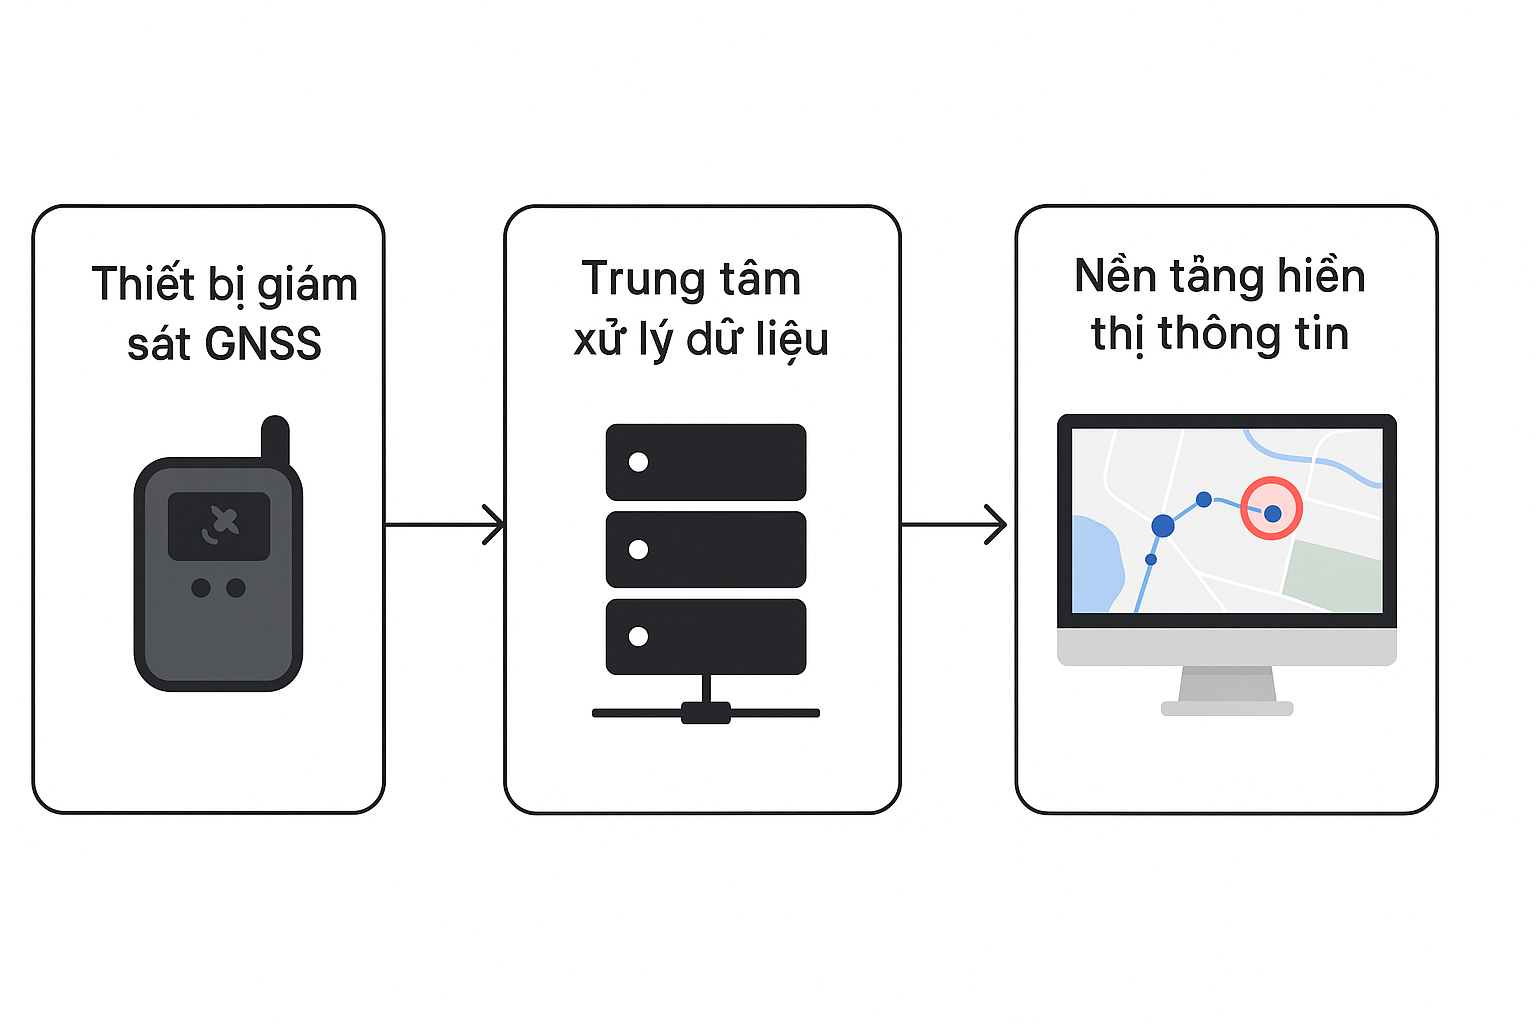
\includegraphics[width=\linewidth]{Hinhve/system_diagram.png}
    \caption{Sơ đồ hệ thống}
    \label{fig:label}
\end{figure}
\subsection{Lựa chọn công nghệ và nền tảng}
\label{subsection:2.2.2}
Việc lựa chọn công nghệ và nền tảng phù hợp là yếu tố quan trọng để đảm bảo hệ thống giám sát và geofence hoạt động ổn định, hiệu quả và đáp ứng các yêu cầu kỹ thuật đã đề ra. Trong hệ thống này, các công nghệ được sử dụng sẽ bao gồm công nghệ định vị GNSS, nền tảng IoT để thu thập và quản lý dữ liệu, cũng như các giao thức truyền thông để kết nối các thành phần.

Công nghệ định vị GNSS đóng vai trò cốt lõi trong việc xác định vị trí của đối tượng. Các hệ thống định vị phổ biến hiện nay như GPS, GLONASS, Galileo và BeiDou đều có những ưu điểm riêng về độ chính xác, độ phủ sóng và khả năng hoạt động trong các điều kiện địa lý khác nhau. Dựa trên điều kiện triển khai và yêu cầu giám sát, hệ thống của tôi sử dụng công nghệ GPS vì độ phổ biến cao, khả năng định vị tốt và tương thích với nhiều thiết bị IoT hiện có.

Để đảm bảo khả năng giám sát và quản lý thiết bị từ xa, nền tảng IoT được lựa chọn là ThingsBoard. Đây là nền tảng mã nguồn mở, cung cấp nhiều tính năng mạnh mẽ như quản lý thiết bị, thu thập dữ liệu, giám sát trực quan và phát hiện sự kiện. ThingsBoard hỗ trợ giao thức truyền thông MQTT và HTTP, giúp tích hợp dễ dàng với các thiết bị IoT. Việc lựa chọn nền tảng này cũng giúp giảm chi phí phát triển và đảm bảo khả năng mở rộng trong tương lai.

Trong hệ thống giám sát, việc truyền tải dữ liệu vị trí từ thiết bị đến trung tâm xử lý là một bước quan trọng. Để đảm bảo tính ổn định và độ trễ thấp, giao thức MQTT được sử dụng làm phương tiện truyền thông chính. MQTT là giao thức nhẹ, phù hợp cho các ứng dụng IoT có băng thông hạn chế và yêu cầu truyền tải dữ liệu liên tục. Nhờ cơ chế Publish/Subscribe, hệ thống có thể gửi và nhận thông tin một cách nhanh chóng, đảm bảo độ tin cậy trong giám sát thời gian thực.

Ngoài ra, để đảm bảo tính bảo mật trong việc truyền tải dữ liệu, hệ thống sử dụng mã hóa TLS (Transport Layer Security) để bảo vệ các gói tin trên nền tảng MQTT. Việc mã hóa này giúp đảm bảo tính toàn vẹn của dữ liệu, tránh nguy cơ bị giả mạo hoặc tấn công từ bên ngoài. Đồng thời, cơ chế xác thực hai lớp (Two-Factor Authentication) cũng được tích hợp để đảm bảo chỉ những thiết bị đã đăng ký mới có thể kết nối với hệ thống.

Đối với việc lưu trữ và xử lý dữ liệu, cơ sở dữ liệu thời gian thực TimescaleDB được lựa chọn do khả năng xử lý lượng lớn dữ liệu định vị với tốc độ cao. TimescaleDB tương thích với PostgreSQL, cung cấp khả năng phân tích dữ liệu lịch sử và giám sát hiệu năng. Điều này rất quan trọng trong việc lưu trữ lộ trình di chuyển và phát hiện các xu hướng bất thường.

Tóm lại, hệ thống giám sát GNSS và geofence được xây dựng dựa trên sự kết hợp của công nghệ GPS, nền tảng ThingsBoard và giao thức truyền thông MQTT. Bằng cách sử dụng các công nghệ hiện đại và nền tảng mạnh mẽ, hệ thống đảm bảo khả năng giám sát liên tục, bảo mật cao và dễ dàng mở rộng trong các ứng dụng thực tế.
\subsection{Đánh giá tính khả thi}
\label{subsection:2.2.3}
Việc đánh giá tính khả thi của hệ thống giám sát là một bước quan trọng nhằm đảm bảo hệ thống có thể đáp ứng các yêu cầu kỹ thuật cũng như phù hợp với thực tiễn triển khai. Trong quá trình đánh giá, các yếu tố như độ chính xác định vị, độ ổn định của hệ thống, khả năng mở rộng và tính bảo mật sẽ được xem xét một cách toàn diện.

Độ chính xác là yếu tố cốt lõi của mọi hệ thống giám sát GNSS. Với việc sử dụng công nghệ GPS, độ chính xác của hệ thống phụ thuộc vào nhiều yếu tố như điều kiện thời tiết, vị trí địa lý và môi trường xung quanh. Qua quá trình thử nghiệm thực tế, thiết bị GNSS cho thấy khả năng định vị với độ sai lệch từ 5 đến 10 mét trong điều kiện thông thường. Trong các môi trường đô thị dày đặc hoặc địa hình phức tạp, độ chính xác có thể giảm xuống đáng kể. Để khắc phục vấn đề này, hệ thống sử dụng các thuật toán lọc nhiễu và bù sai số như Kalman Filter, giúp cải thiện độ tin cậy của vị trí định vị.

Độ ổn định của hệ thống được đánh giá thông qua khả năng duy trì kết nối liên tục giữa thiết bị giám sát GNSS và nền tảng ThingsBoard. Các thử nghiệm cho thấy việc sử dụng giao thức MQTT giúp duy trì kết nối ổn định với độ trễ trung bình dưới 1 giây khi truyền tải dữ liệu định vị. Trong các trường hợp mất kết nối tạm thời, hệ thống tự động thực hiện cơ chế tái kết nối mà không làm gián đoạn quá trình giám sát. Điều này đảm bảo dữ liệu luôn được cập nhật kịp thời, đặc biệt quan trọng trong các tình huống yêu cầu giám sát liên tục.

Một trong những ưu điểm của hệ thống là khả năng mở rộng dễ dàng khi cần giám sát nhiều đối tượng cùng lúc. Với việc sử dụng nền tảng ThingsBoard, hệ thống có thể quản lý hàng trăm thiết bị mà không làm giảm hiệu năng. Cơ chế phân phối dữ liệu theo chủ đề (topic) của MQTT giúp việc xử lý dữ liệu từ nhiều nguồn diễn ra đồng thời mà không gây xung đột. Bên cạnh đó, cơ sở dữ liệu TimescaleDB hỗ trợ lưu trữ lượng lớn dữ liệu định vị trong thời gian dài, giúp việc phân tích lịch sử di chuyển trở nên hiệu quả.

Tính bảo mật của hệ thống được đảm bảo thông qua việc áp dụng các cơ chế mã hóa và xác thực chặt chẽ. Dữ liệu định vị từ thiết bị đến nền tảng ThingsBoard được mã hóa bằng TLS, ngăn chặn việc đánh cắp thông tin trong quá trình truyền tải. Ngoài ra, việc sử dụng xác thực hai lớp (2FA) giúp đảm bảo rằng chỉ những thiết bị được đăng ký trước mới có quyền truy cập vào hệ thống. Điều này giúp hạn chế nguy cơ bị xâm nhập hoặc giả mạo từ bên ngoài.

Thông qua các thử nghiệm ban đầu, hệ thống cho thấy khả năng giám sát liên tục với độ chính xác cao, đặc biệt là trong môi trường mở. Khả năng mở rộng và tính bảo mật được đảm bảo nhờ lựa chọn công nghệ và nền tảng phù hợp. Tuy nhiên, một số thách thức như độ trễ khi tín hiệu yếu hoặc mất kết nối vẫn cần được cải thiện.

Nhìn chung, hệ thống giám sát được thiết kế với sự chú trọng đến độ chính xác, độ ổn định, khả năng mở rộng và bảo mật. Các yếu tố này đã được thử nghiệm và cho kết quả khả quan trong điều kiện thực tế. Việc lựa chọn công nghệ hiện đại, nền tảng ThingsBoard và giao thức MQTT giúp hệ thống đạt được hiệu năng mong muốn, đồng thời đảm bảo tính bảo mật cao trong quá trình triển khai. Các kết quả đánh giá tính khả thi sẽ là nền tảng để tiến hành các bước thiết kế chi tiết và triển khai hệ thống trong thực tế.
\end{document}